\begin{comment}
\end{comment}

\chapter{Construction de codes correcteurs quantiques}

Dans le chapitre précédent, 
je me suis intéressé à la correction des erreurs lors de la communication classique.
Pour la suite de la thèse,
je quitterai ce régime pour m'intéresser au régime quantique.
Dans ce chapitre, 
je m'intéresserai plus particulièrement à la protection de l'information 
dans un modèle quantique simplifié avant de présenter la conception d'une mémoire 
quantique au prochain chapitre.
Ce modèle simplifié ressemble au canal binaire symétrique présenté au premier chapitre
et il permet d'étudier la construction de codes correcteurs d'erreurs quantiques sans prendre en compte les détails d'implémentation.

De façon semblable au scénario classique,
concevoir des codes correcteurs qui permettent de bien protéger l'information avec un nombre raisonnable de qubits supplémentaires est crucial.
En fait,
la présence des erreurs est l'un des obstacles parmi les plus
limitants pour la réalisation de calculs quantiques.
Ainsi, 
la correction d'erreurs ne se limite pas à des scénarios de communication 
comme dans le cas classique,
mais sera omniprésente dans un système de calcul quantique.

Cette importance accrue des erreurs dans les systèmes quantiques s'explique
principalement du fait qu'il s'agit de systèmes analogues plutôt que digitaux.
Un système est digital lorsque chacun de ses éléments peut prendre un nombre fini
de valeurs. 
Dans le cas des ordinateurs classiques,
chaque bit prend soit la valeur 0 ou la valeur 1.
Ainsi,
une quantité continue comme une différence de potentiel représente physiquement un bit tout en le protégeant des erreurs.
Par exemple,
le bit 0 peut être associé à une valeur de 0 volt et le bit 1 à une valeur de 5 volts.
Dans le cas où une valeur de 4.9 volts serait mesurée, il est fort probable que 
la valeur désirée était le bit 1.
Donc, en absence des perturbations externes présentent lors de la communication,
l'information classique est relativement robuste.

Au contraire, un système quantique est analogue puisqu'il existe une infinité d'états accessibles.
Par exemple, toutes paires de nombres complexes $a$ et $b$ telles que $a^2 + b^2 = 1$
représentent l'état d'un qubit.
Ainsi, 
une faible variation de ces paramètres représente un état différent
et distinguer l'état désiré d'un état corrompu est généralement impossible.
De plus, l'accumulation de ces petites différences peut complètement
changer le résultat d'un calcul.

Ces erreurs émergent généralement de processus de décohérence.
Par exemple,
un système quantique dans un état excité tend naturellement à retourner dans un état de moindre énergie.
Au milieu des années 1990,
plusieurs scientifiques croyaient que
les erreurs engendrées par la décohérence des systèmes quantiques
représentaient un obstacle insurmontable au calcul quantique~\cite{unruh_maintaining_1995, palma_quantum_1996, landauer_is_1995, chuang_quantum_1995}.
Leurs arguments reposaient entre autres sur le théorème de non-clonage~\cite{wootters_single_1982}
stipulant qu'il est impossible de copier l'état d'un qubit vers un second qubit.
Cela semblait donc empêcher l'utilisation de la redondance pour 
protéger le système des erreurs comme c'est le cas pour la communication classique.

Nous savons aujourd'hui comment contourner ces limitations. 
Les premiers à avoir proposé une solution sont Calderbank, Shor et Steane~\cite{calderbank_good_1996, steane_multiple-particle_nodate}.
D'ailleurs, à la prochaine section,
je vais introduire une importante famille de codes correcteurs quantiques, les codes CSS, qui porte leur nom.
En réponse à ce résultat, Gottesman~\cite{gottesman_stabilizer_1997} a introduit le formalisme des codes stabilisateurs
que je vais utiliser dans ce chapitre pour décrire les codes correcteurs quantiques.

Depuis,
plusieurs familles de codes correcteurs quantiques ont été introduites.
Les codes les plus étudiés sont sans aucun doute les codes de surfaces et 
les codes toriques introduits par Kitaev~\cite{kitaev_fault-tolerant_2003}.
Cependant,
ces codes, bien qu'excellent pour protéger le système,
ne permettent pas d'encoder efficacement un grand nombre de qubits~\cite{bravyi_tradeoffs_2010}.
Pour contrer ce problème,
les codes quantiques d'opérateurs de parité à faible 
densité~(LDPC, de l'anglais \textit{low-density parity-check})
reçoivent de plus en plus d'attention.
Cet intérêt est en partie stimuler par le succès des codes LDPC classiques introduient
par Gallager~\cite{gallager_low-density_1962}.
De plus, il a été montré par Gottesman~\cite{gottesman_fault-tolerant_2013}
qu'il est possible d'utiliser des codes quantiques LDPC pour 
construire des ordinateurs quantiques protégés des erreurs avec 
un surcoût constant en qubits.
Il s'agit donc d'outils importants pour la réalisation du calcul quantique à grand échelle.

Les codes quantiques LDPC incluent plusieurs familles,
dont les codes par produit d'hypergraphes~\cite{tillich_quantum_2014}
et les codes par produit homologique~\cite{bravyi_homological_2014}.
Comme l'indique le nom de ces exemples,
les codes quantiques LDPC sont généralement obtenus par le produit 
de structures associées à des codes correcteurs classiques.
Dans le cadre de cette thèse,
j'ai conçu une approche qui permet plutôt de générer des codes correcteurs quantiques
directement,
sans avoir recours à une construction classique au préalable.
L'un des principaux avantages de cette méthode est sa flexibilité 
lors de la construction des codes.
En fait,
cette construction permet de générer n'importe quelle famille de codes stabilisateurs
dont les codes LDPC.

Cette approche repose sur la résolution d'un problème de satisfication de contraintes.
Bien que ce problème soit généralement difficile à résoudre,
j'ai numériquement identifié des régimes pour lesquels il est aisé de
construire des codes correcteurs quantiques
et des régimes pour lesquels la tâche est beaucoup plus ardue.
Cela, bien que surprenant, est un comportement attendu pour ce type de problème.

Je reviendrai sur ce fait plus loin dans ce chapitre
après avoir présenteré le formaliste des canaux bruités quantiques 
et des codes stabilisateurs.
Finalement,
je présenterai l'article expliquant la construction et 
mettant de l'avant les résultats de ce projet.

\section{Correction d'erreurs quantique}

\subsection{Canaux bruités quantiques}

Un état quantique est généralement représenté par un opérateur de densité $\rho$
de trace unité.
Une évolution arbitraire d'un état $\rho$ vers un état $\rho'$
c'est-à-dire une combinaison d'opérations unitaires,
de mesures et d'interactions avec l'environnement, 
est représentée par une application
\begin{align}
  \rho' = \mathcal{E}(\rho).
\end{align}
Pour décrire plus précisément cette transformation,
j'utiliserai les opérateurs de Krauss.
Dans ce cas,
l'application est définie comme
\begin{align}
  \mathcal{E}(\rho) = \sum_{k} E_k \rho E_k^\dag,
\end{align}
avec la condition que 
\begin{align}
  \sum_k E_k^\dag E_k = I.
\end{align}
Cette dernière permet d'assurer que $\tr(\mathcal{E}(\rho)) = 1$.

Dans leur excellent livre d'introduction à l'informatique quantique de 
Neilsen et Chuang~\cite{nielsen_quantum_2010} motivent en détails 
cette définition générale pour l'évolution d'un état quantique.
Ainsi, je me limite à une justification intuitive de cette définition
et j'invite les personnes intéressées à consulter le huitième chapitre de ce livre.

De façon générale,
l'état $\rho$ évolue au sein d'un environnement dont les états de bases 
sont $\qty{\ket{e_0}, \ket{e_1}, \ldots}$.
Au début d'une expérience (ou d'un calcul),
le système et l'environnement sont dans un état de produit tensoriel,
c'est-à-dire, un état sans intrication.
De plus, il est suffisant de considérer que l'environnement est dans l'état 
pur $\ket{e_0}$.
En effet,
si ce n'est pas le cas, il suffit de choisir un environnement plus grand jusqu'à 
obtenir un état pur.
Ainsi,
l'état initial du système et de l'environnement est $\rho \otimes \op{e_0}$.

Par la suite,
un opérateur unitaire $U$ est appliqué sur le système et l'environnement suivit d'une
mesure de l'environnement sans connaitre le résultat.
Le circuit correspondant est illustré à la figure~\ref{fig:circuit_canal_quantique}.
Ainsi, l'état final du système est
\begin{equation}
  \mathcal{E}(\rho) 
  = \tr_{\text{env}}\qty(U(\rho \otimes \op{e_0})U^\dag)
  = \sum_k \bra{e_k}U(\rho \otimes \op{e_0}) U^\dag \ket{e_k}
  = \sum_k E_k \rho E_k^\dag
\end{equation}
avec $E_k = \mel{e_k}{U}{e_0}$.
Ainsi,
l'application $\mathcal{E}$ représente la transformation de l'état d'un système quantique
lorsque celui-ci intéragit avec son environnement et que l'on ignore l'état final
de l'environnement.

Une autre interprétation est suite à l'application $\mathcal E$,
le système se retrouve dans l'état $\rho_k \propto E_k \rho E_k^\dag$
avec probabilité $p_k = \tr(E_k \rho E_k^\dag)$.
Il est alors possible d'écrire l'application comme
\begin{align}
  \mathcal E(\rho) = \sum_k p_k \rho_k.
\end{align}
Cette formulation montre clairement l'utilité de $\mathcal E$ pour
représenter un canal bruité quantique.
De façon similaire à un canal bruité classique,
un canal quantique transforme un premier état 
vers un second état choisi aléatoirement.

Dans cette thèse,
je me limite aux canaux bruités quantiques avec des opérateurs 
de Krauss $E_k$ proportionnels aux opérateurs de Pauli.
Les opérateurs de Pauli pour un seul qubit sont 
\begin{align}
  &I = \op{0}{0} + \op{1}{1}, 
  &&Y = -i\op{0}{1} + i\op{1}{0}, \notag \\
  &X = \op{0}{1} + \op{1}{0}, 
  &&Z = \op{0}{0} - \op{1}{1}.
\end{align}
Le groupe~\footnote{Je fais un rappel des notions de théorie des groupes à l'annexe~\ref{chap:theo_groupes}}
de Pauli $\mathcal P_n$ de $n$ qubits est un groupe multiplicatif sur 
l'ensemble des opérateurs $\qty{I, X, Y, Z}^n$ avec une phase parmi $\qty{1, i, -1, -i}$.
Dans ce cas,
le canal s'écrit généralement comme
\begin{align}
  \mathcal E(\rho) = \sum_{Q \in \mathcal P_n} p_Q Q\rho Q.
\end{align}


\begin{figure}
  \begin{center}
    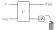
\includegraphics{figures/circuit_canal_quantique.pdf}
  \end{center}
  \caption[Représentation en circuit d'un canal quantique]{
    Représentation en circuit d'un canal quantique.
    Le résultat de la mesure est ignoré.
  }
  \label{fig:circuit_canal_quantique}
\end{figure}




\subsection{Codes stabilisateurs}

L'une des meilleures ressources pour une présentation complète du formalisme des codes
stabilisateurs est la thèse de doctorat de Gottesman~\cite{gottesman_stabilizer_1997}.
Dans cette section,
je me limiterai plutôt aux concepts essentiels à la compréhension des travaux et de l'article associé.



\subsection{Théorème du seuil et évaluation de la performance des codes correcteurs quantiques}




\section{Problèmes de satisfaction de contraintes}
\subsection{Transition de phases et seuil de satisfiabilité}

\section{Article : Une multitude de codes stabilisateurs éparses}

Cet article soumis au journal Quantum à l'été 2022 a pour titre original
\textit{Finite-rate quantum sparse codes aplenty}.
Celui-ci était toujours en processus de révision lors de la soumission de cette thèse.

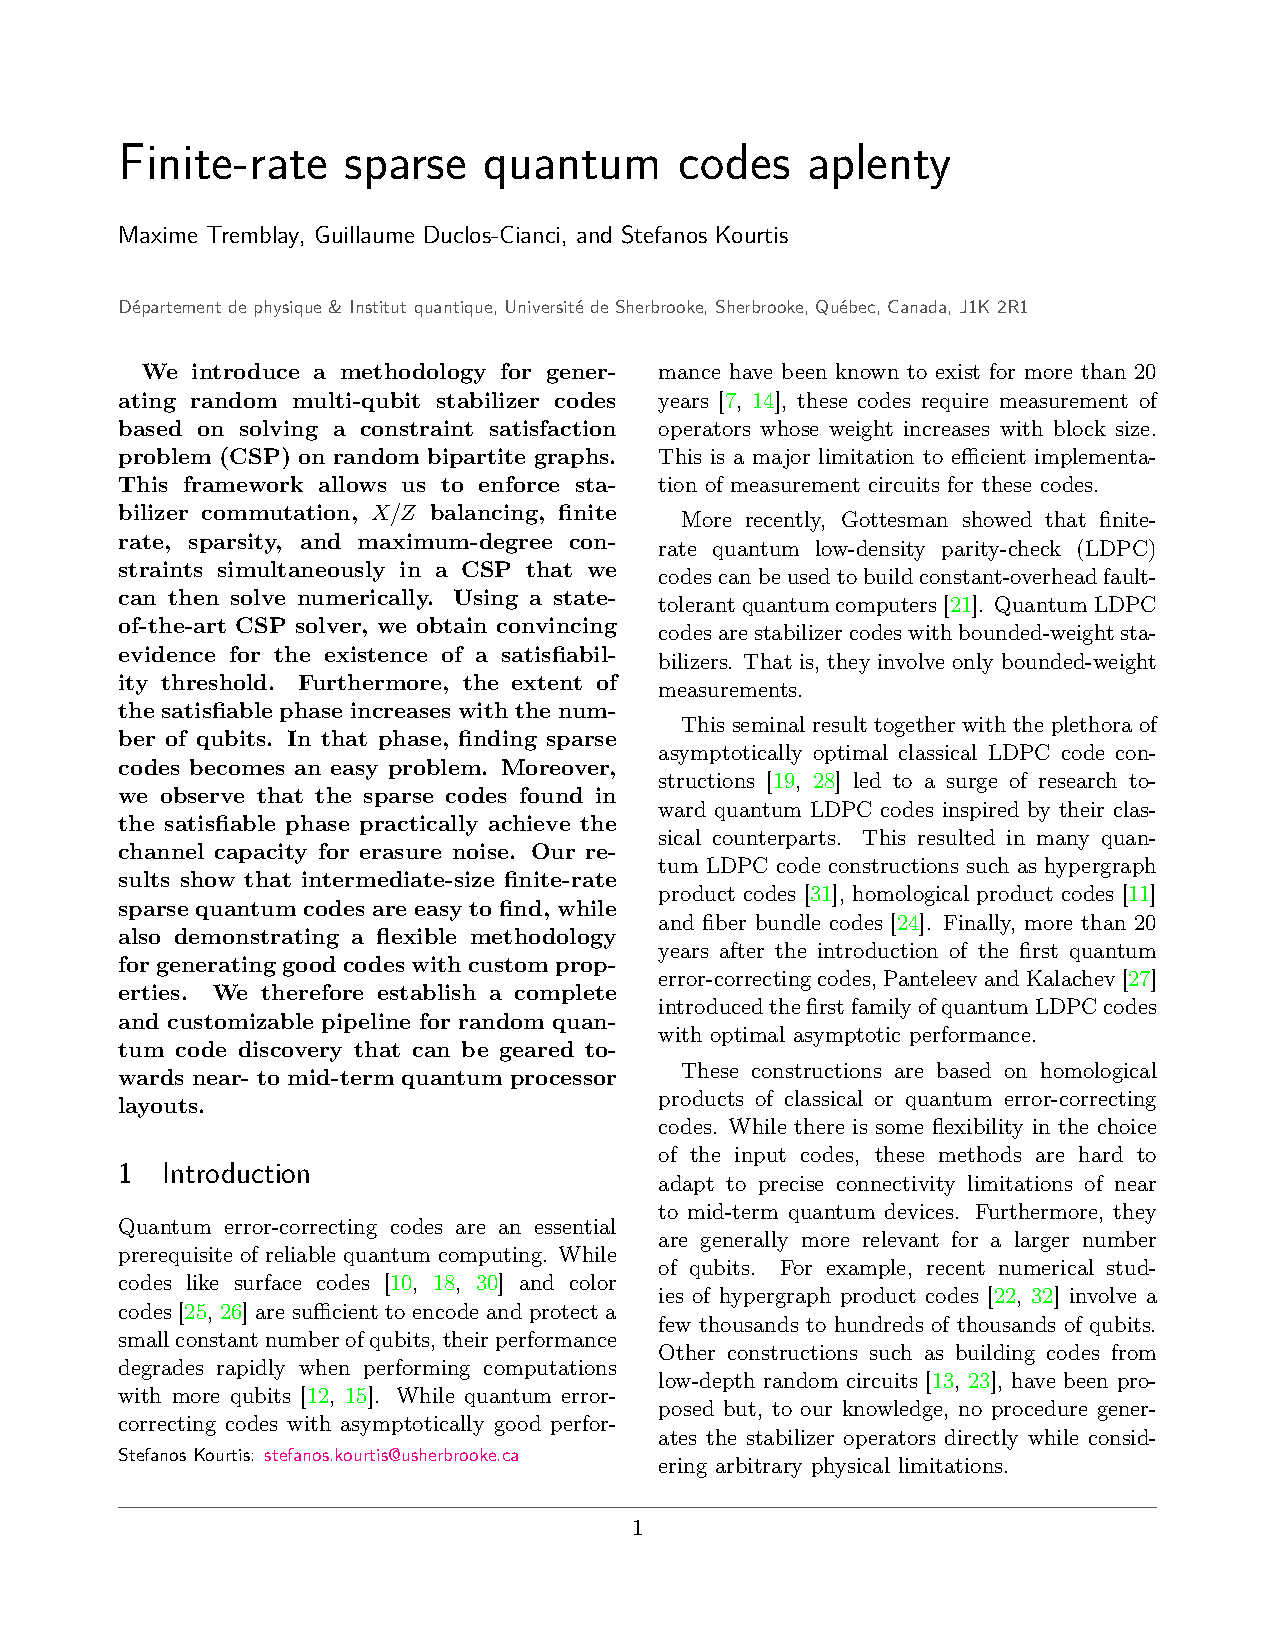
\includepdf[pages=-]{articles/sat_codes_construction.pdf}
